\documentclass[a4paper,11pt]{article}

%%%%%%%%%
%%usees%%
%%%%%%%%%
\usepackage[utf8]{inputenc}
%\usepackage[ngerman]{babel}
%\usepackage{a4wide}
\usepackage[margin=3.0cm, top=3.0cm, bottom=3.0cm]{geometry}
\usepackage{setspace}
\usepackage{graphicx}
\usepackage{amssymb} 
\usepackage{amsmath}
\usepackage{mathtools}
\usepackage{footnote}
\usepackage{caption}
\usepackage{color}
\usepackage[hidelinks]{hyperref}
\usepackage{cite}
\usepackage{todonotes}


\newcommand{\reffig}[1]{Figure~\ref{#1}}

%%%%%%%%%
%%Title%%
%%%%%%%%%

\author{Frederik Zwilling 304314}
\title{Master-Thesis Proposal:\\ Shared Robot Memory for Multiple Planners in Fawkes}
\begin{document}
%\thispagestyle{empty}
%\tableofcontents
%\newpage
%\onehalfspace
\maketitle
%%%%%%%%%
%%Text%%
%%%%%%%%

\abstract{abstract.}

\section{Introduction}
\label{sec:introduction}
\begin{itemize}
\item Motivation Knowledge Representation on Cyber Physical Systems
\item Problem description
  \begin{itemize}
  \item Worldmodel exchange between resoners/planners
  \item Worldmodel exchange between robots
  \item Long time storage
  \end{itemize}
\item Idea Robot Memory
\item Application RCLL PDDL-CLIPS
\item Application @Home/PR2
\end{itemize}

\section{Background}
\label{sec:background}
This section presents the background of the proposed thesis. On the
one hand, we describe the primary application and evaluation domain,
the RoboCup with the RoboCup Logistics League (RCLL), the @Home league
and their robots in ~\ref{sec:robocup}. On the other hand, we present
the most important software for the proposed thesis. In
section~\ref{sec:fawkes} we present the robot software framework
Fawkes. Section~\ref{sec:planners} describes the planners and
reasoners which should profit from using the robot memory and in
section~\ref{sec:mongodb} MongoDB, the database used in the backend of
the robot memory.

\subsection{RoboCup}
\label{sec:robocup}
\todo[inline]{rewrite or copy from bachelorthesis?}  The
\emph{RoboCup} is an international robotics competition founded to
foster research in the field of robotics and artificial
intelligence.~\cite{Robocup}. It provides standard problems as a
platform to foster and compare research results. Research
teams from all over the world compete in different leagues to
benchmark their robotic system. The RoboCup provides a research
test-bed, in which participating teams implement new approaches and
make them robust against the challenges of the real world
complexity. Furthermore, the competition leads to comparison and
evaluation of different approaches.\\
%
The RoboCup features a variety of leagues, each focusing on another
aspect or application domain of robotics and artificial
intelligence. The majority of the RoboCup leagues host soccer robots
in different sizes and complexities. The leagues range from the
\emph{Small Size League} with small cylindrical robots and ground
truth perception from an overhead camera to humanoid robots in teen
size which need to have all sensors and computation devices on the
robot. The RoboCup also features more application oriented domains,
e.g. the \emph{Rescue League} with robots solving different
challenges in desaster scenarios and \emph{RoboCup@Work} with robots
operating in an industrial scenario to perform identification,
handling and transporting tasks with work related objects such as
skrews and nuts. The \emph{RoboCup Logistics League (RCLL)} which
features logistics robots in a production scenario and the
\emph{RoboCup@Home} leage featuring service robots in a domestic
environment are presented in the following in more detail because
these two leagues are used as application and evaluation domains of
the proposed thesis.


\subsubsection{RoboCup Logistics League}
\begin{figure}
  \begin{minipage}[b]{0.5\linewidth}
    \centering
    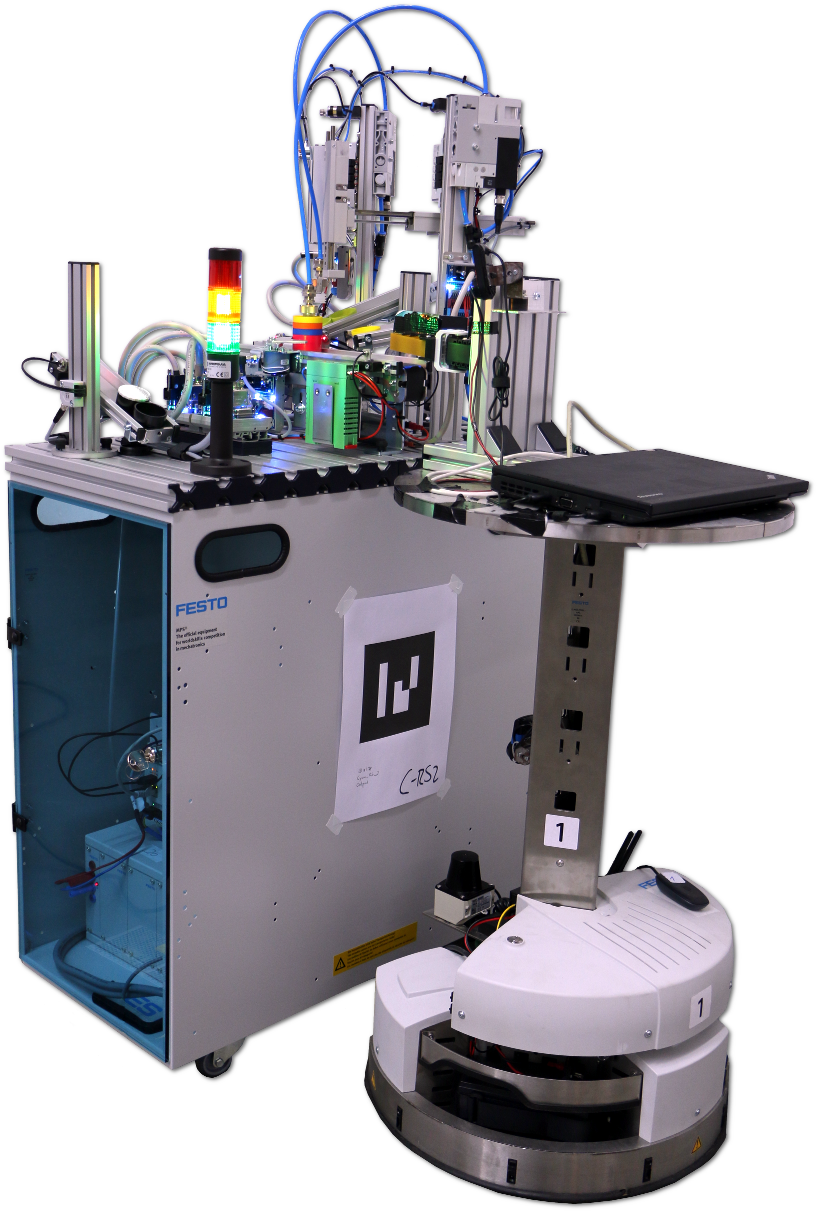
\includegraphics[width=0.5\textwidth]{img/rcll}
    \caption{Robot and MPS used in the RCLL}
    \label{fig:rcll}
  \end{minipage}
\quad
\begin{minipage}[b]{0.5\linewidth}
  \todo[inline]{empty}
  \label{fig:}
\end{minipage}
\end{figure}

\todo[inline]{League, robotino}
%
The \emph{RoboCup Logistics League (RCLL)}\footnote{RoboCup Logistics
  League website: \url{http://www.robocup-logistics.org}}, previously
LLSF, is a industry-oriented competition within RoboCup.  It tackles
the problem of production logistics in a smart factory where mobile
robots have to plan, execute, and optimize the material and production
flow between machines to produce and deliver products according to
dynamic orders. Competing teams deploy a group of up to three robots
which have to autonomously build ordered products by interacting with
\emph{Modular Production Machines (MPS)} and transporting workpieces
between these machines.  \reffig{fig:rcll} shows an RCLL robot filling
a machine which mounts colored rings on workpieces. The robots are
based on the Festo Robotino 3 platform which uses an holonomic drive,
and can be extended and programmed by the teams. The robot shown in
\reffig{fig:rcll} was build by the Carologistics team and used an
laser range finder for localization, a custom made gripper for
handling workpieces and several cameras for detection of AR-tags and
light-signals mounted on the machines~\cite{Carologistics2015}. The
game is controlled by a software component called \emph{referee box
  (refbox)} which randomizes the machine placement in the factory and
the production orders, communicates with the competing robots,
controls the machines and awards points.

The game consists of two phases~\cite{LLSF-Rules-2015}. In the first
phase, the \emph{exploration phase}, the robots have to roam the
factory to find randomly placed machines which are used later. By
detecting the light signal shown by the machines, the robots can
determine the machine-type. For correct reportsof discovered machines
to the refbox the team is awarded points, for incorrect ones points
are subtracted.
%
\begin{figure}[t]
  \centering
  \begin{minipage}{.8\linewidth}
  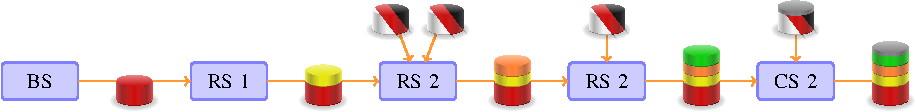
\includegraphics[width=\linewidth]{img/chain_c3}%
  \end{minipage}
  \quad%
  \begin{minipage}{.15\linewidth}
  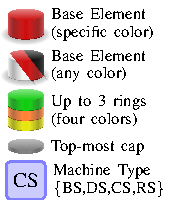
\includegraphics[width=\linewidth]{img/legend}%
  \end{minipage}
  \caption{Production chain of a high complexity
    product in the RCLL.}
  \vspace{-2mm}
  \label{fig:prod-chain}
\end{figure}
%
In the second phase, the \emph{produciton phase}, the refbox announces
orders, which products have to be produced by the robots. The products
are build from colored cups with optionally mounted rings and and a
colored cap. \reffig{fig:prod-chain} shows the production chain to
build a high complexity product. There are four different machine
types. The \emph{base-station (BS)} provides new bases, the colored
cups, as raw ressource. The \emph{ring stations (RS)} mounts colored
rings on a workpiece and after preparing it with a varying amount of
bases. The \emph{cap-station (CS)} mounts black or grey caps to finish
a product after loading it with a cap form a shelf first. The
\emph{delivery-station (DS)} is used to deliver products.

The challenges of the RCLL lie in the dynamic and only partially
observable environment the robots have to robustly and fully
autonomously work in, in the planning and multi-robot coordination
required to build as many ordered products as possible and deliver
them in time given time window, and in the baseline robotic challenges
such as collision avoidance, perception and behavior execution. The
dynamism of the environment is caused by the ranomized factory layout,
randomized out-of-order times of machines, the highly customizable
amount of products that preclude producing in advance, unknown
obstacles, such as the other teams robots and hard to completely avoid
handling mistakes by the robots. To cope with these challenges and
achieve an efficient production, a multi-robot decision making is
nesseccary.

\subsubsection{@Home League}
\todo[inline]{League, Ceasar}

%% The RoboCup@Home league is a
%% competition about service robots. The robots have to assist humans in
%% a domestic environment. There are a variety of tasks, such as
%% following a human, serving drinks and handling emergency
%% situations. Especially important in this league are the technical and
%% open challenge. Here, the teams can present their own ideas and how
%% the robot implements them.

\subsection{Fawkes Robot Software Framework}
\label{sec:fawkes}
%% \begin{itemize}
%% \item Component based approach
%% \item Blackboard
%% \item Comparison to ROS
%% \end{itemize}


\subsection{Planners and Reasoners}
\label{sec:planners}
\begin{itemize}
\item CLIPS
\item PDDL
\item Golog
\item MoveIt
\end{itemize}
\subsection{MongoDB}
\label{sec:mongodb}
\begin{itemize}
\item MongoDB
\item Query Language
\item Comparison to using CLIPS, KnowRob
\item Comparison to other DBs (SQL, Graph DBs, other Document DBs)
\end{itemize}

\section{Related Work}
\label{sec:related}
\subsection{KnowRob}
\label{sec:knowrob}
\begin{itemize}
\item Common sense Resoning
\item Concepts Ontologies, Triple Store, Virtual Knowledge base
\item Prolog implementation
\item Pro/Contra
\end{itemize}
\subsection{OpenRobots Ontology (ORO)}
\begin{itemize}
\item Events (Trigger)
\item RDF, Ontologies
\item multi-agent?
\end{itemize}
\subsection{MongoDB Logging}
\label{sec:mongo-logging}
\subsection{More}
\todo[inline]{More}
\begin{itemize}
\item Blackboard
\item RoboEarth
\item Robot Memory... Robot Databases... Robot Knowledge Storage...
\end{itemize}


\section{Approach}
\label{sec:approach}
\subsection{Goals}
\label{sec:goals}
\begin{itemize}
\item Same worldmodel for reasoners/planners
\item Distributed for robot team
\item Long time storage (persistent, different kinds of long time knowledge, decay?)
\item Triggers
\item Interrupt storage?
\item Beliefs/Confidences?
\item Versatility (virtual knowledge base)
\item Temporal/Spatial grounding
\item Common sense knowledge
\end{itemize}
\subsection{Architecture}
\label{sec:arch}
\begin{itemize}
\item Data representation
\item Component interactions (diagram)
\item Middle-layer (virtual kb resolving)
\item Data acquisition
\end{itemize}


\subsection{Implementation}
\label{sec:impl}
\subsubsection{Robot Memory}
\label{sec:impl-memory}
\begin{itemize}
\item Data Representation
\item MongoDB query language
\item Trigger
\item Multi-robot synchronization
\end{itemize}
\subsubsection{Planner/Reasoner}
\label{sec:impl-planner}
\begin{itemize}
\item Example for using the Robot Memory
\item Queries/Register Triggers
\item Build initial domain
\item When to replan
\end{itemize}

\subsection{Evaluation}
\label{sec:eval}
\subsubsection{Application}
\label{sec:eval-apl}
\begin{itemize}
\item RCLL PDDL-CLIPS
\item RCLL between bots
\item @Home
\end{itemize}
\subsubsection{Efficiency-Scalability}
\subsubsection{Expressiveness}
\subsubsection{Versatility}
\subsubsection{Software development expandability, interfacing}
\subsection{Schedule}
\begin{itemize}
\item Timetable
\end{itemize}

\section{Summery}
\label{sec:summery}
\begin{itemize}
\item Challenges
\item Impact
\end{itemize}


\bibliographystyle{plain}
\bibliography{../references}

\end{document}
